\section{Methods}

The proposed method is a deployment gate for selecting demand-planning strategies. Figure~\ref{fig:framework} shows the gate: candidate forecasts and policies are converted into planning signals, scored for feasibility, and then approved or rejected for deployment. This design follows forecast-to-decision research showing that downstream operational quality can differ from forecast-error quality (Elmachtoub and Grigas 2022; Mandi et al. 2024).

\begin{figure}[htbp]
\centering
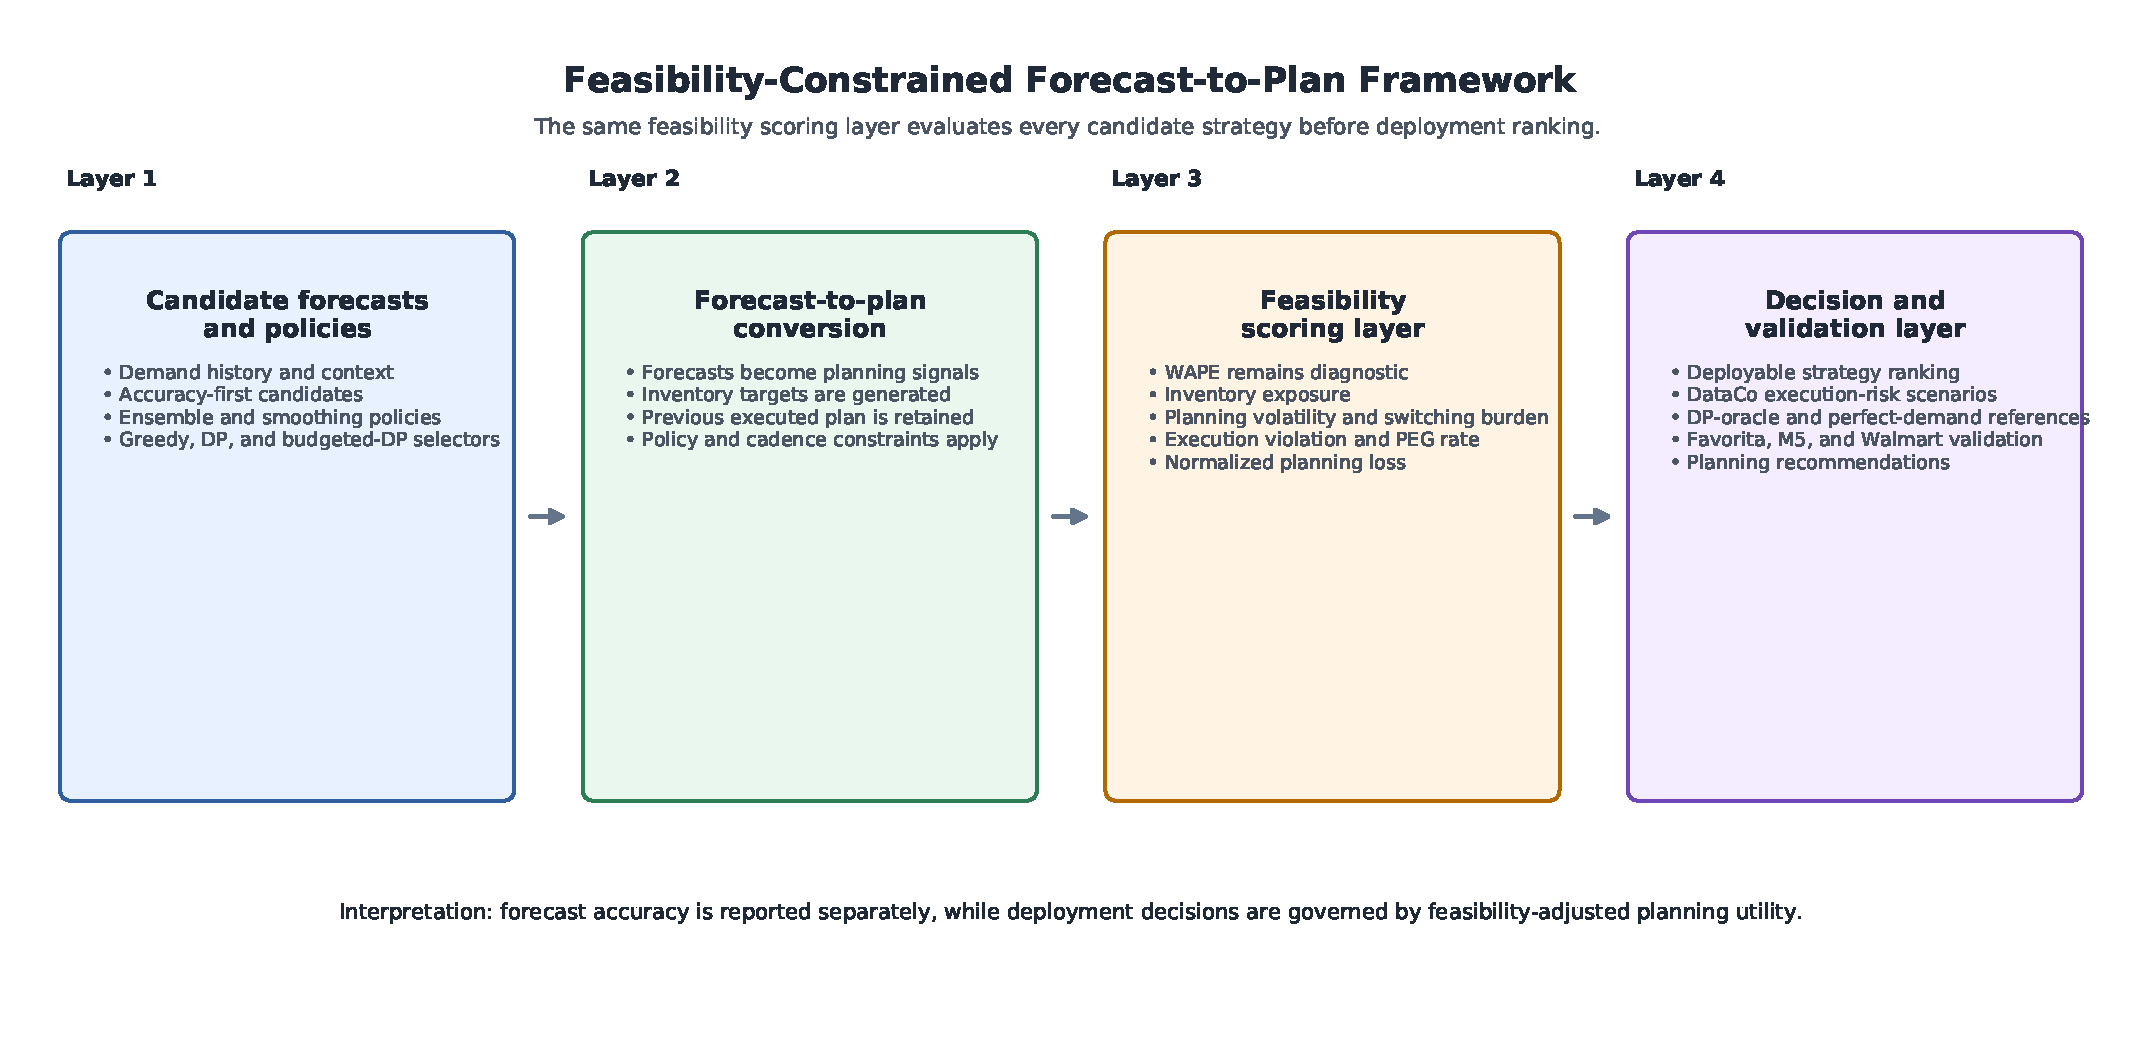
\includegraphics[width=0.96\linewidth]{figures/ieom_framework_flowchart.pdf}
\caption{Forecast-to-plan feasibility gate for demand-planning deployment.}
\label{fig:framework}
\end{figure}

Figure~\ref{fig:framework} is a deployment gate, not only a workflow. WAPE remains visible as a diagnostic signal, but the approval decision is governed by whether the forecast-driven plan can be operationally executed.

\subsection{Forecast-to-plan Feasibility Model}

Let $i$ index a planning unit, $t$ index a planning period, and $m$ index a candidate forecasting model or planning policy. The candidate forecast is $\hat{y}_{i,t}^{m}$, and the executable planning signal is $p_{i,t}^{m}$. The forecast-to-plan conversion is:
\begin{equation}
p_{i,t}^{m}=g(\hat{y}_{i,t}^{m},\mathrm{policy}_{t}).
\end{equation}
In this study, the planning signal is an inventory target implied by the candidate forecast and planning policy.

Inventory exposure is measured using holding and shortage terms:
\begin{equation}
IC_{i,t}^{m}=h[p_{i,t}^{m}-y_{i,t}]^{+}+b[y_{i,t}-p_{i,t}^{m}]^{+},
\end{equation}
where $h$ is holding cost, $b$ is shortage cost, $y_{i,t}$ is realized demand, and $[x]^+=\max(x,0)$.

Planning volatility and execution violation are:
\begin{equation}
PV_{i,t}^{m}=|p_{i,t}^{m}-p_{i,t-1}|,
\end{equation}
\begin{equation}
EV_{i,t}^{m}=[|p_{i,t}^{m}-p_{i,t-1}|-C_{i,t}]^{+},
\end{equation}
where $C_{i,t}$ is the execution capacity available to absorb plan movement. The planning-execution gap rate for strategy $s$ is:
\begin{equation}
PEG(s)=\frac{1}{T}\sum_{t=1}^{T}\mathbb{I}\{EV_t(s)>0\}.
\end{equation}

The normalized planning loss is:
\begin{align}
L(s)={}&
\beta_{\mathrm{inventory}}\cdot \mathrm{NIC}(s)
+\lambda_{\mathrm{volatility}}\cdot \mathrm{NVC}(s) \notag \\
&+\lambda_{\mathrm{execution}}\cdot \mathrm{NEC}(s)
+\lambda_{\mathrm{switch}}\cdot \mathrm{NSC}(s),
\end{align}
where NIC, NVC, NEC, and NSC are normalized inventory, volatility, execution, and switching components. WAPE is reported separately as diagnostic forecast accuracy. The main operational objective excludes direct forecast-error terms because realized inventory exposure and feasibility terms capture the deployable consequences of forecast-driven planning decisions.

\subsection{Stepwise Feasibility-constrained Selection Algorithm}

\textbf{Algorithm 1. Feasibility-constrained selection procedure.}

\begin{enumerate}
\item Generate candidate forecasts or planning policies for each planning unit and period.
\item Convert each candidate forecast into a planning signal.
\item Compute inventory exposure relative to realized demand.
\item Compute planning volatility and switching burden relative to the previous executed plan.
\item Compute execution violation under the available execution capacity.
\item Aggregate the normalized planning loss.
\item Select the deployable planning action using one of the decision policies.
\item Validate the selected strategy against scenario and oracle benchmarks.
\end{enumerate}

Steps 1--3 create candidate planning signals. Steps 4--6 score those signals by feasibility. Step 7 selects a deployment action. Step 8 validates whether the action remains preferred under execution-risk scenarios and oracle benchmarks. The procedure is modular: accuracy-first baselines, ensembles, smoothing rules, greedy selectors, DP selectors, and budgeted-DP selectors all pass through the same forecast-to-plan feasibility gate.

\subsection{Horizon-aware and Constrained Selection}

The greedy selector minimizes the current-period operational cost. Let $c_t(m_{t-1},m)$ denote the validation-derived stage cost of choosing candidate $m$ after previous model $m_{t-1}$. The greedy selector chooses:
\begin{equation}
m_t^{G}=\arg\min_{m\in\mathcal{M}} c_t(m_{t-1},m).
\end{equation}

The finite-horizon DP selector accounts for future transition effects:
\begin{equation}
V_t(m_{t-1})=\min_{m\in\mathcal{M}}\{c_t(m_{t-1},m)+V_{t+1}(m)\},
\end{equation}
with terminal condition $V_{T+1}(\cdot)=0$. The greedy-to-DP gap measures myopic selection suboptimality. When this gap is small, one-step selection may be adequate; when switching approval and coordination costs are material, DP provides a planning-ahead benchmark.

The budgeted DP selector adds a governance constraint:
\begin{equation}
\sum_{t=2}^{T}\mathbb{I}\{m_t\neq m_{t-1}\}\leq K.
\end{equation}
The state includes the previous model and the number of switches already used. Transitions exceeding the switch budget are discarded. If missing candidate availability leaves no feasible path, the implementation uses a flagged incumbent-stays fallback that is budget-compliant when the incumbent model remains available.

Smoothing represents gradual operational adaptation:
\begin{equation}
p_t=\alpha p_t^{\mathrm{candidate}}+(1-\alpha)p_{t-1}.
\end{equation}
Lower $\alpha$ values reduce execution burden but can delay response to demand changes. Ensemble policies combine candidate forecasts and are evaluated as low-disruption alternatives when accuracy remains comparable.

\subsection{Validation Benchmarks}

The Realized-Inventory Oracle DP is non-deployable. It uses realized test-period inventory outcomes over the same forecast candidates and measures the value of unavailable inventory-outcome information. The DP-oracle gap measures selection suboptimality relative to this non-deployable benchmark.

The Perfect-Demand Oracle is also non-deployable. It uses realized demand as the planning signal and is a perfect-demand diagnostic reference, not a guaranteed lower bound. Exact demand tracking can increase planning volatility and execution violations when the operation cannot absorb rapid plan movement. The perfect-demand reference gap therefore measures a diagnostic total gap that includes both forecast uncertainty and feasibility effects.
